\documentclass[11pt, a4paper]{article}

% --- ESSENTIAL PACKAGES ---

% Font Encoding and Input
\usepackage[T1]{fontenc} % Use 8-bit T1 fonts to ensure proper character rendering
\usepackage[utf8]{inputenc} % Allows direct use of UTF-8 characters (e.g., é, ö, à)
\usepackage{amsmath} % For \text{} in math mode

% Page Layout and Margins
\usepackage{geometry}
\geometry{
    a4paper,
    left=2.5cm,
    right=2.5cm,
    top=3cm,
    bottom=3cm
}

% Professional Fonts (Latin Modern)
\usepackage{lmodern}
\usepackage{helvet} % For Helvetica font, used for the main title

% --- COLOR AND STYLING ---

% Color Management
\usepackage[dvipsnames]{xcolor} % Use dvipsnames for a wider range of predefined colors

% Define a professional color palette
\definecolor{primary}{HTML}{0A369D}  % A deep, professional blue
\definecolor{secondary}{HTML}{4472CA} % A lighter, complementary blue
\definecolor{darkgray}{HTML}{333333}  % For body text, better than pure black
\definecolor{customgreen}{HTML}{5E8B7E} % A muted green for accents
\definecolor{titleblue}{HTML}{082A75} % A darker, rich blue for the main title

\color{darkgray} % Set the default text color

% Section and Title Styling
\usepackage{titlesec}
\titleformat{\section}
  {\normalfont\Large\bfseries\color{primary}} % Format for the section title
  {\thesection}{1em}{} % Section number, spacing, and the title itself
\titleformat{\subsection}
  {\normalfont\large\bfseries\color{secondary}}
  {\thesubsection}{1em}{}
\titleformat{\subsubsection}
  {\normalfont\bfseries\color{customgreen}}
  {\thesubsubsection}{1em}{}

% --- IMAGES AND GRAPHICS ---

% Standard package for including images
\usepackage{graphicx}
\graphicspath{{images/}} % Optional: specify a folder for your images
\usepackage{float} % Improved control over figure placement with [H] option

% --- LISTS AND ENUMERATIONS ---

% Customize list environments
\usepackage{enumitem}
% The 'textcolor' option sets the color for the item's text
\setlist[itemize,1]{label=\textcolor{primary}{\textbullet}}
\setlist[itemize,2]{label=\textcolor{secondary}{\textendash}}

% --- HYPERLINKS ---

% Hyperlink styling for URLs and cross-references
\usepackage{hyperref}
\hypersetup{
    colorlinks=true,
    linkcolor=primary,
    filecolor=magenta,
    urlcolor=secondary,
    citecolor=customgreen,
    pdftitle={My Professional Document},
    pdfpagemode=FullScreen,
}

% --- TYPOGRAPHY AND MICRO-ADJUSTMENTS ---

% Improves the justification and spacing of text for a cleaner look
\usepackage{microtype}

% --- DOCUMENT CONTENT EXAMPLE ---

% For placeholder text
\usepackage{lipsum}

% --- TABLE AND CURRENCY PACKAGES ---
\usepackage{booktabs} % For professional looking tables
\usepackage{longtable} % For tables that may span multiple pages
\usepackage{siunitx} % For aligning numbers in tables
\usepackage{eurosym} % For the EUR symbol
\usepackage{float} % to use [H]

\title{A Causal AI Framework for Longitudinal Modelling of Prostate Cancer}
\author{Project Acronym: CausalPCa}
\date{}

\begin{document}

\maketitle

\section{Excellence}

\subsection{Vision: A Paradigm Shift from Prediction to Causal Understanding}
Prostate cancer (PCa) represents a paramount public health challenge, ranking as the second most common cancer in men worldwide \cite{CaraccioloCastello2024,DulleaOSullivan2025}. In 2020 alone, over 1.4 million new cases were diagnosed globally, and it stands as the fifth leading cause of cancer-related death among men, responsible for approximately 375,000 deaths that year \cite{CereserEvangelista2023,GammelSolari2024,DharCendejasGomez2024}. The epidemiological trajectory is alarming, with projections indicating that the number of cases will more than double to 2.9 million by 2040, driven largely by an aging global population \cite{UdovicichJia2025,SungFerlay2021}.

The management of PCa is fraught with complexity, stemming from the dual risks of overdiagnosis and undertreatment. Widespread screening with prostate-specific antigen (PSA) has led to the frequent detection of indolent, clinically insignificant cancers, resulting in overtreatment and significant morbidity \cite{PadhaniSchoots2023,JenaTaneja2018,CaraccioloCastello2022}. Conversely, many PCa deaths are due to the late diagnosis of aggressive or metastatic disease \cite{PadhaniSchoots2023}. The stakes of misstaging are incredibly high; the distinction between localized and metastatic disease carries profound prognostic implications, with the 5-year survival rate dropping from nearly 100\% to as low as 30-40\% \cite{WangODwyer2024,CereserEvangelista2023}.

This diagnostic dilemma is exacerbated by the limitations of current AI models. While they have shown promise, they operate as sophisticated but dangerously opaque "black boxes." They excel at identifying statistical correlations but fundamentally lack a true understanding of the underlying causal biology of the disease. This critical gap fosters mistrust and creates a barrier to clinical adoption, as models can be easily misled by spurious correlations—such as scanner artifacts, site-specific protocols, or population biases—leading to predictions that are brittle, unexplainable, and potentially unsafe.

We put forward a radical new vision for clinical AI, a paradigm shift from simple prediction to deep causal reasoning. We aim to build not just another predictive tool, but a dynamic, interactive "digital twin" of a patient's disease trajectory. Our goal is to create a model that understands the intricate cause-and-effect relationships driving cancer progression, can simulate future outcomes under different treatment scenarios, and can explain its reasoning through clinically intuitive counterfactuals. By enabling a clinician to ask "what if...?"—\textit{what would this scan have looked like if this patient had been treated with Lutetium-PSMA therapy six months ago? What if this suspicious lesion were benign?}—we empower them with a tool that augments their own reasoning process, transforming the model from a black box into a trusted collaborator.

This project does not aim to incrementally improve existing methods; it aims to forge the technology-to-come. It is a high-risk, high-gain endeavor to create a foundational, causal framework that will not only revolutionize prostate cancer care but will also establish a new European standard for trustworthy, explainable, and safe medical AI.

\subsection{Consortium and Clinic Expertise}
Our consortium is uniquely positioned to succeed in this high-risk, high-gain endeavor. The applicant clinic, the Universitätsklinik für Radiologie und Nuklearmedizin, possesses not only the requisite multimodal data but also a proven track record in developing and deploying advanced AI models in a clinical setting. Our team has successfully executed projects involving:
\begin{itemize}
    \item \textbf{Synthetic Image Generation:} We have hands-on experience in generating synthetic CT scans from PET data, a foundational skill for the generative components of this proposal.
    \item \textbf{Predictive Modeling:} Our team has developed and validated models for predicting disease progression by fusing clinical and imaging data, directly relevant to the core of this project.
    \item \textbf{Clinical Application Development:} We have created a user-friendly GUI for structured reporting and developed an LLM-based support application for thyroid cancer guidelines, demonstrating our ability to translate research into practical clinical tools.
\end{itemize}
Crucially, the project will be led by a team that includes members with rare dual expertise, holding degrees in both medicine (MD with a specialization in nuclear medicine) and IT (PhD). This unique leadership structure ensures a seamless bridge between the complex technical development and the real-world clinical needs and validation requirements, a critical success factor for a project of this ambition. The collaboration with the Abteilung für Nuklearmedizin at Universitätsmedizin Halle further strengthens our consortium, providing diverse data and clinical perspectives.

\subsection{Objectives}
This project is guided by a set of clear, ambitious, and interconnected objectives designed to realize our vision of a causal AI for prostate cancer, directly aligning with the Pathfinder's goal of developing foundational, high-impact technologies. The primary objectives are:
\begin{enumerate}
    \item \textbf{To Pioneer a Causal, Longitudinal Model of Prostate Cancer:} The core scientific objective is to develop and validate a novel Causal AI framework, built upon a Neural Jump Ordinary Differential Equation (NJDE) architecture. This model will be capable of learning the underlying dynamics of disease progression from sparse, irregularly-sampled, multi-modal data, while explicitly modeling the impact of clinical interventions like surgery and therapy. This foundational technology will establish a new European standard for clinical AI.

    \item \textbf{To Achieve True Explainability through Counterfactual Reasoning:} We will move beyond opaque "black-box" models by building a system that can generate clinically plausible, visual counterfactuals. This will enable clinicians to ask "what-if" questions and receive intuitive, visual explanations for the model's predictions, fostering the clinical trust necessary for widespread adoption and establishing a new paradigm for trustworthy AI.

    \item \textbf{To Master Heterogeneity through Principled Disentanglement:} A key technical objective is to develop a robust Variational Autoencoder (VAE) framework that can disentangle the core components of medical imaging data. The model will learn to separate true disease signals from patient-specific anatomy, age-related changes, and technical confounders (e.g., scanner type, site-specific artifacts), ensuring the model is robust, generalizable, and ready for deployment across diverse European healthcare systems.

    \item \textbf{To Create a Dynamic "Digital Twin" for Personalized Prognosis:} We aim to deliver a tool that can simulate a patient's future disease trajectory under various scenarios. The model will generate predictions not only of future scans but also of key clinical endpoints and structured radiological reports, providing a comprehensive, personalized prognostic tool that has the potential to revolutionize patient management.

    \item \textbf{To Quantify Uncertainty for Safer Clinical Decisions:} We will develop and integrate robust methods for uncertainty quantification directly into our framework. The model will not only provide predictions but also a reliable measure of its own confidence, a critical feature for safe clinical use. This allows the system to "know what it doesn't know," flagging high-uncertainty cases for closer human review and preventing over-reliance on automated outputs.
    \item \textbf{To Validate the Framework in a Real-World Clinical Context:} The project will culminate in a rigorous evaluation of the model's performance, using both quantitative metrics (e.g., predictive accuracy, counterfactual quality) and a qualitative, clinician-in-the-loop study to assess its real-world clinical plausibility, utility, and impact on diagnostic workflows, thereby paving the way for its integration into the European healthcare ecosystem.
\end{enumerate}

\subsection{Concept and Methodology: A Feasible Path to a Groundbreaking Technology}
Our methodology is a direct answer to the profound challenges of building trustworthy clinical AI. We have designed a novel, \textbf{four-stage causal framework} that deconstructs the immense complexity of prostate cancer progression into a series of well-defined, manageable tasks. This modular approach is the key to our project's feasibility: it ensures training stability, enhances model interpretability, and allows us to systematically embed clinical domain knowledge as strong inductive biases. This guides the model to learn the true underlying causal mechanisms of the disease, rather than superficial correlations. This design leverages our consortium's extensive experience in synthetic image generation (CT from PET) and predictive modeling, and is illustrated in Figure \ref{fig:ml_framework}.

\begin{figure}[H]
    \centering
    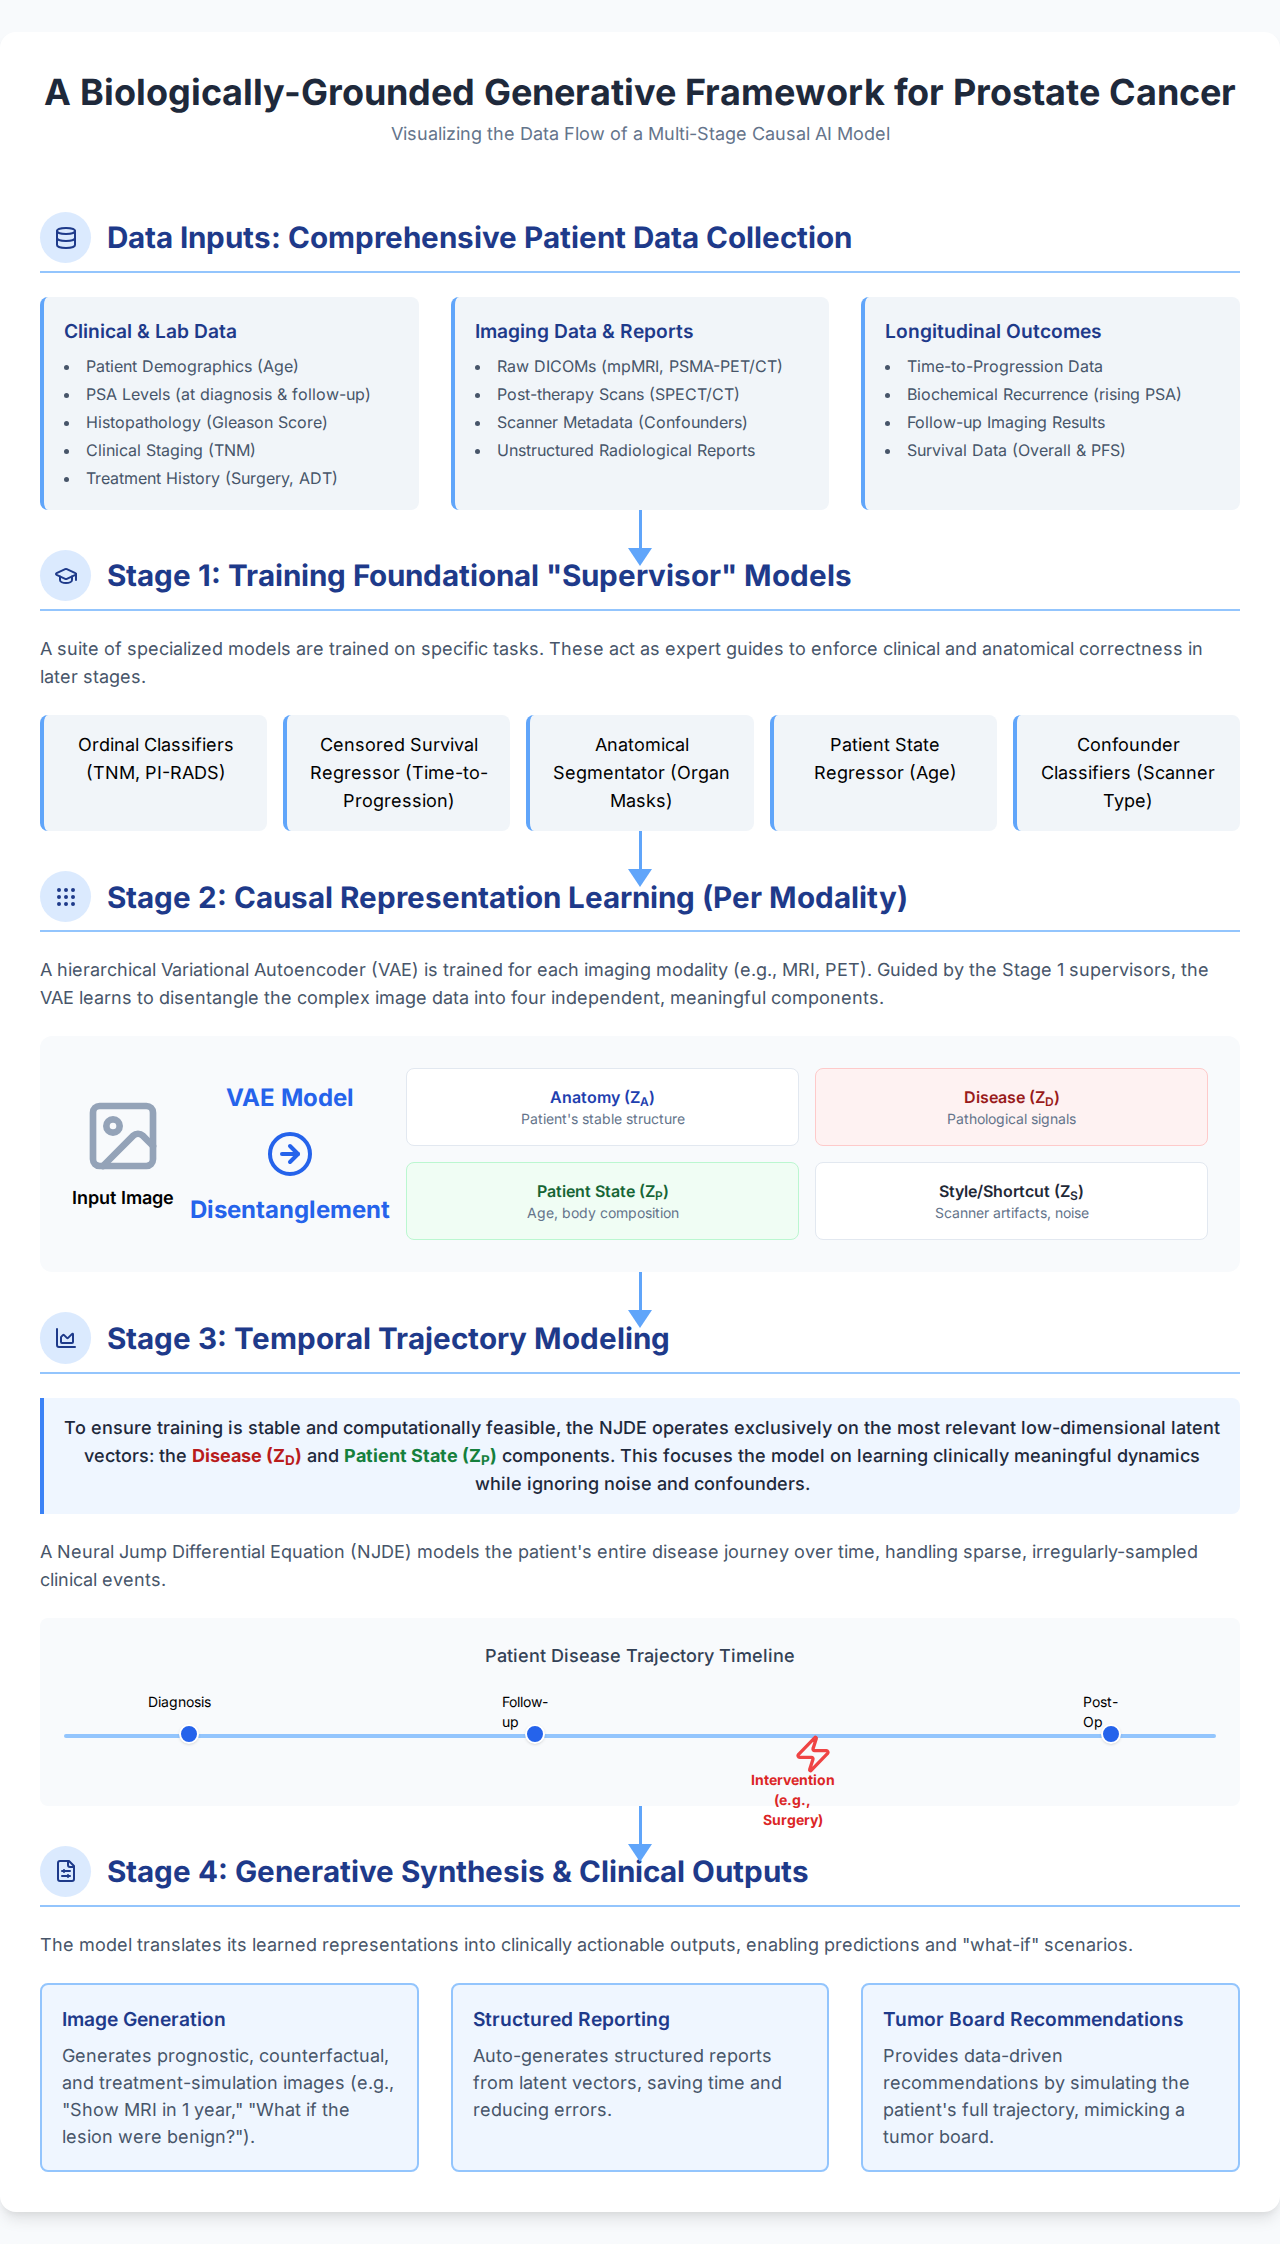
\includegraphics[width=\textwidth]{ml.png}
    \caption{Data flow diagram of the proposed multi-stage causal AI model. The process begins with comprehensive patient data, which is used to train foundational supervisor models. These guides inform a per-modality VAE to learn a disentangled latent space. A Neural Jump ODE then models the patient's temporal disease trajectory from these latent representations, culminating in generative outputs like prognostic images and structured reports.}
    \label{fig:ml_framework}
\end{figure}

\subsubsection{Stage 1: Building the Bedrock of Clinical Validity with Supervisor Models}
The first stage builds a suite of specialized "supervisor" models. These models act as expert guides, providing strong, clinically-validated signals that will enforce a valid structure on the more complex generative models in subsequent stages. Our team's prior success in developing predictive models from fused clinical and imaging data provides a strong foundation for this work package.
\begin{itemize}
    \item \textbf{Ordinal Classifiers:} For clinical scores with an inherent order (e.g., PI-RADS, TNM stage), standard categorical classifiers are suboptimal. We will implement a \textbf{differential ordinal learning framework} that explicitly encodes the ordered structure by combining a standard categorical loss with a differential ordinal loss, ensuring the model understands that a higher grade implies a worse prognosis \cite{LeeByeon2025, GrisiKartasalo2025}.
    \item \textbf{Censored Survival Regressor:} To predict time-to-progression (TTP), we will train a survival model that properly handles right-censored data. This will be achieved using a censored regression loss (e.g., Logistic Hazard) combined with a ranking loss regularizer (e.g., SurvRNC) to ensure correct risk ordering in the learned feature representation \cite{GaoLi2019, RivailVogl2023, ShahinZhao2023}.
    \item \textbf{Anatomical and Confounder Models:} We will fine-tune a pre-trained TotalSegmentator model to provide anatomical ground truth. Furthermore, we will train dedicated regressors and classifiers to predict patient age, BMI, and technical confounders (e.g., scanner type, dosage, data source location), allowing us to explicitly model and isolate these non-disease-related sources of variation and ensure the model generalizes well across geographically different patient populations \cite{PuglisiAlexander2025, ZhangHager2025}.
\end{itemize}

\subsubsection{Stage 2: Mastering Heterogeneity through Principled Disentanglement}
At the heart of our solution to data heterogeneity is a hierarchical Variational Autoencoder (VAE) trained for each imaging modality to learn a disentangled latent space. The key innovation is partitioning this space into four independent, semantically meaningful components: Anatomy ($Z_A$), Disease ($Z_D$), Patient State ($Z_P$), and Style/Confounders ($Z_S$). This separation is enforced through a composite loss function:
$$ \mathcal{L}_{\text{total}} = \mathcal{L}_{\text{VAE}} + \lambda_A \mathcal{L}_{\text{Anatomy}} + \lambda_D \mathcal{L}_{\text{Disease}} + \lambda_I \mathcal{L}_{\text{Disentangle}} $$
The disentanglement is achieved by moving beyond simple $\beta$-VAE approaches. Our loss function will apply a \textbf{targeted penalization} of the statistical dependence between latent subspaces. We recognize that some correlations are clinically meaningful (e.g., disease can affect anatomy), while others are spurious. Therefore, the model will be heavily penalized for mutual information between causally independent subspaces (e.g., Disease $Z_D$ and Style $Z_S$, which includes scanner type and data source), while allowing for natural correlations between dependent factors like disease and anatomy. This is accomplished by selectively applying a Total Correlation (TC) penalty, ensuring the learned disease representation is invariant to technical artifacts without sacrificing the reconstruction of clinically valid relationships \cite{FragemannArdizzone2022, AbbasiMonadjemi2018, FayCobos2023}. The entire data curation and preprocessing pipeline is visualized in Figure \ref{fig:data_curation}.

\begin{figure}[H]
    \centering
    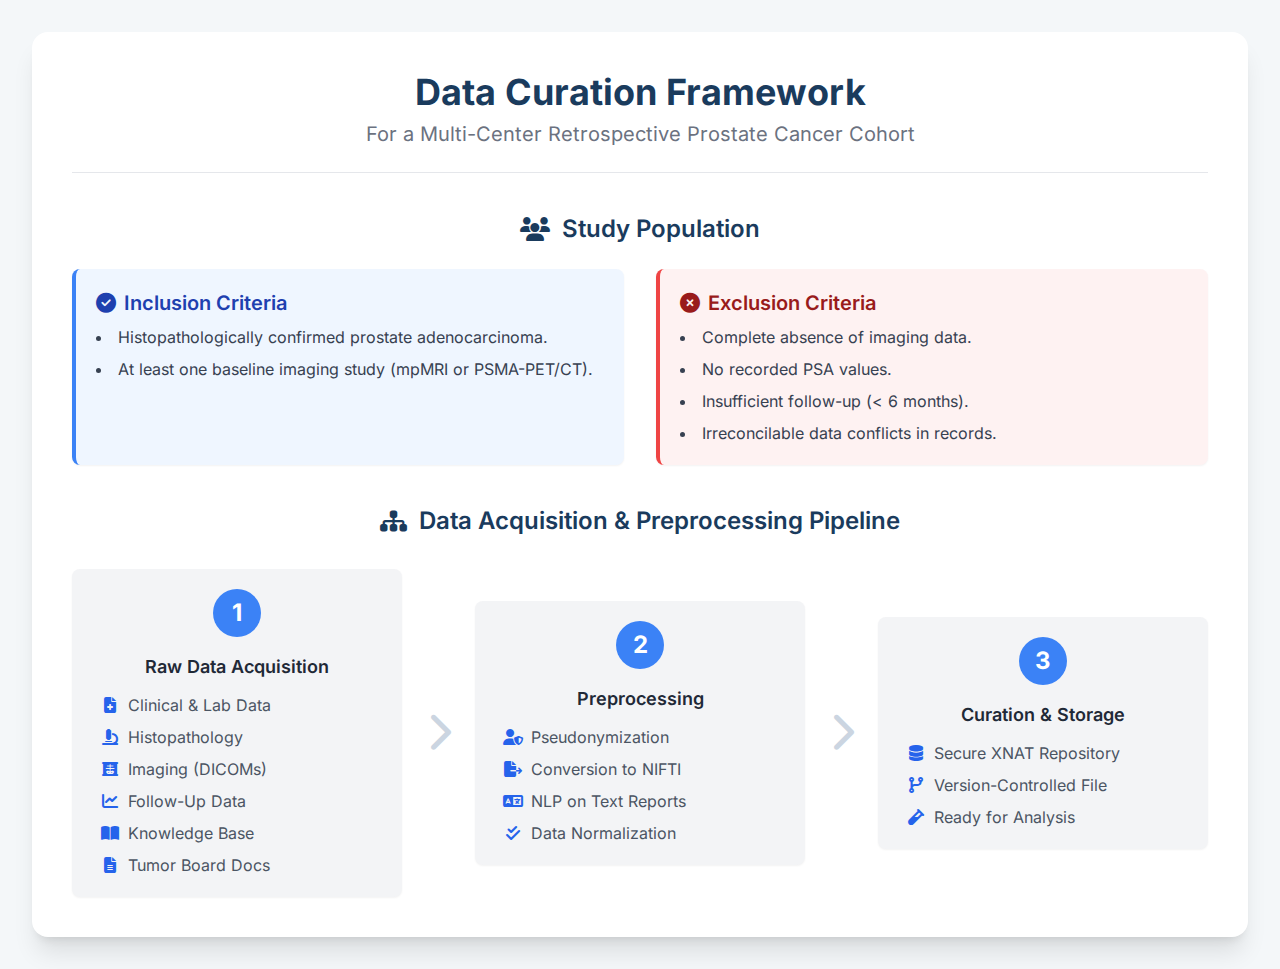
\includegraphics[width=\textwidth]{dc.png}
    \caption{An infographic summarizing the data acquisition, curation, and preprocessing framework for the study cohort. It details the inclusion and exclusion criteria for patient selection and outlines the multi-step pipeline for processing clinical, histopathological, and imaging data.}
    \label{fig:data_curation}
\end{figure}

\subsubsection{Stage 3: Capturing Disease Dynamics with Neural Jump ODEs}
This stage confronts the critical challenge of modeling disease evolution from sparse, multimodal, and irregularly-sampled clinical data. Our solution is a \textbf{Neural Jump Differential Equation (NJDE)} framework, which is uniquely suited for this task \cite{GwakSim2020}.

\paragraph{Rationale and Latent State Formulation}
Neural Ordinary Differential Equations (NODEs) are powerful because they model system dynamics in continuous time, making them inherently robust to irregular sampling—a defining characteristic of clinical data \cite{GwakSim2020, JohnsonBulgarelli2023, BelogolovskyGreenberg2023}. However, their primary weakness is the extreme computational cost of applying them directly to high-dimensional data like 3D images \cite{WiewelBecher2018, DavisChoromanski2020}. Our approach strategically mitigates this by operating exclusively on the low-dimensional latent spaces learned in Stage 2. This is not just an efficiency gain; thanks to the successful disentanglement, we do not need to pass the entire latent space to the temporal model. Instead, by training the NODE only on the most relevant parts—the disentangled \textbf{disease ($Z_D$) and patient state ($Z_P$) components}—we focus the model on learning the dynamics of disease progression itself, making the learning task more tractable and clinically relevant \cite{AshmanSo2020, KberKalisch2023, LosadaTerranova2024}.

The input for the NJDE is a carefully constructed time series of latent state vectors. For each patient, we define a unified state vector $\mathbf{v}$ that has a fixed shape, representing a concatenation of all possible inputs. The process is as follows:
\begin{enumerate}
    \item \textbf{Unified State Vector Definition:} A canonical tensor shape is defined for a state vector $\mathbf{v}$, which includes dedicated slots for the disease latent code ($Z_D$) and patient state code ($Z_P$) from each imaging modality (MRI, PET, SPECT), and for embeddings of all non-imaging data (PSA, clinical note embeddings, etc.).
    \item \textbf{Time-stamped Sparse Tensor Creation:} For each time point $t_i$ where a patient has data, a new state vector $\mathbf{v}(t_i)$ is created and initialized with zeros. The available data is then placed into its corresponding slot in the tensor. For example, at a time point with a PET scan and PSA value, only the $Z_{D_{\text{PET}}}$, $Z_{P_{\text{PET}}}$, and PSA embedding slots are filled, while all other slots remain zero.
    \item \textbf{Anatomy Vector Storage:} The patient-specific anatomy vectors ($Z_A$) from each imaging study are not included in the dynamic state vector but are stored separately, indexed by time, for use in the final image reconstruction stage.
\end{enumerate}
This procedure yields a dataset of sparse, irregularly-sampled latent state vectors, providing a computationally efficient and robust representation of each patient's unique clinical history.

\paragraph{NJDE Training and Dynamics}
The NJDE learns the rules of disease evolution by modeling two phenomena \cite{GwakSim2020}:
\begin{itemize}
    \item \textbf{Continuous Evolution (The NODE):} Between clinical events, the disease state evolves smoothly. This is modeled by a classic NODE that learns the underlying dynamics from the sparse state vectors \cite{BergHasenclever2018}.
    $$ \frac{d\mathbf{v}(t)}{dt} = f(\mathbf{v}(t), t; \psi) \quad \text{for } t \neq t_k $$
    \item \textbf{Discrete Jumps (The Interventions):} At the specific time $t_k$ of a clinical intervention (e.g., prostatectomy, initiation of hormonal therapy), the continuous evolution is interrupted by a discrete "jump." A separate neural network, $g$, models this instantaneous change to the state vector based on the type of intervention \cite{CuchieroLarsson2019, AbushaqraXue2022}.
    $$ \mathbf{v}^+ = g(\mathbf{v}(t_k), \text{intervention}_k; \phi) \quad \text{for } t = t_k $$
\end{itemize}
This hybrid approach, which explicitly separates the continuous disease course from the rapid, external impacts of clinical interventions, is critical for accurately modeling a patient's journey \cite{GwakSim2020}. The model is trained using a \textbf{leave-one-out strategy} for each patient's time series: given all but one time point, its goal is to predict the complete state vector for the held-out time point. To handle the pervasive missing data, we employ a \textbf{masked loss function}. The loss is calculated only by comparing the predicted values to the ground truth for those elements of the state vector that were actually available (non-zero) at the target time point. This forces the model to learn a probable evolution for every data type, even from a highly incomplete dataset.

\begin{figure}[H]
    \centering
    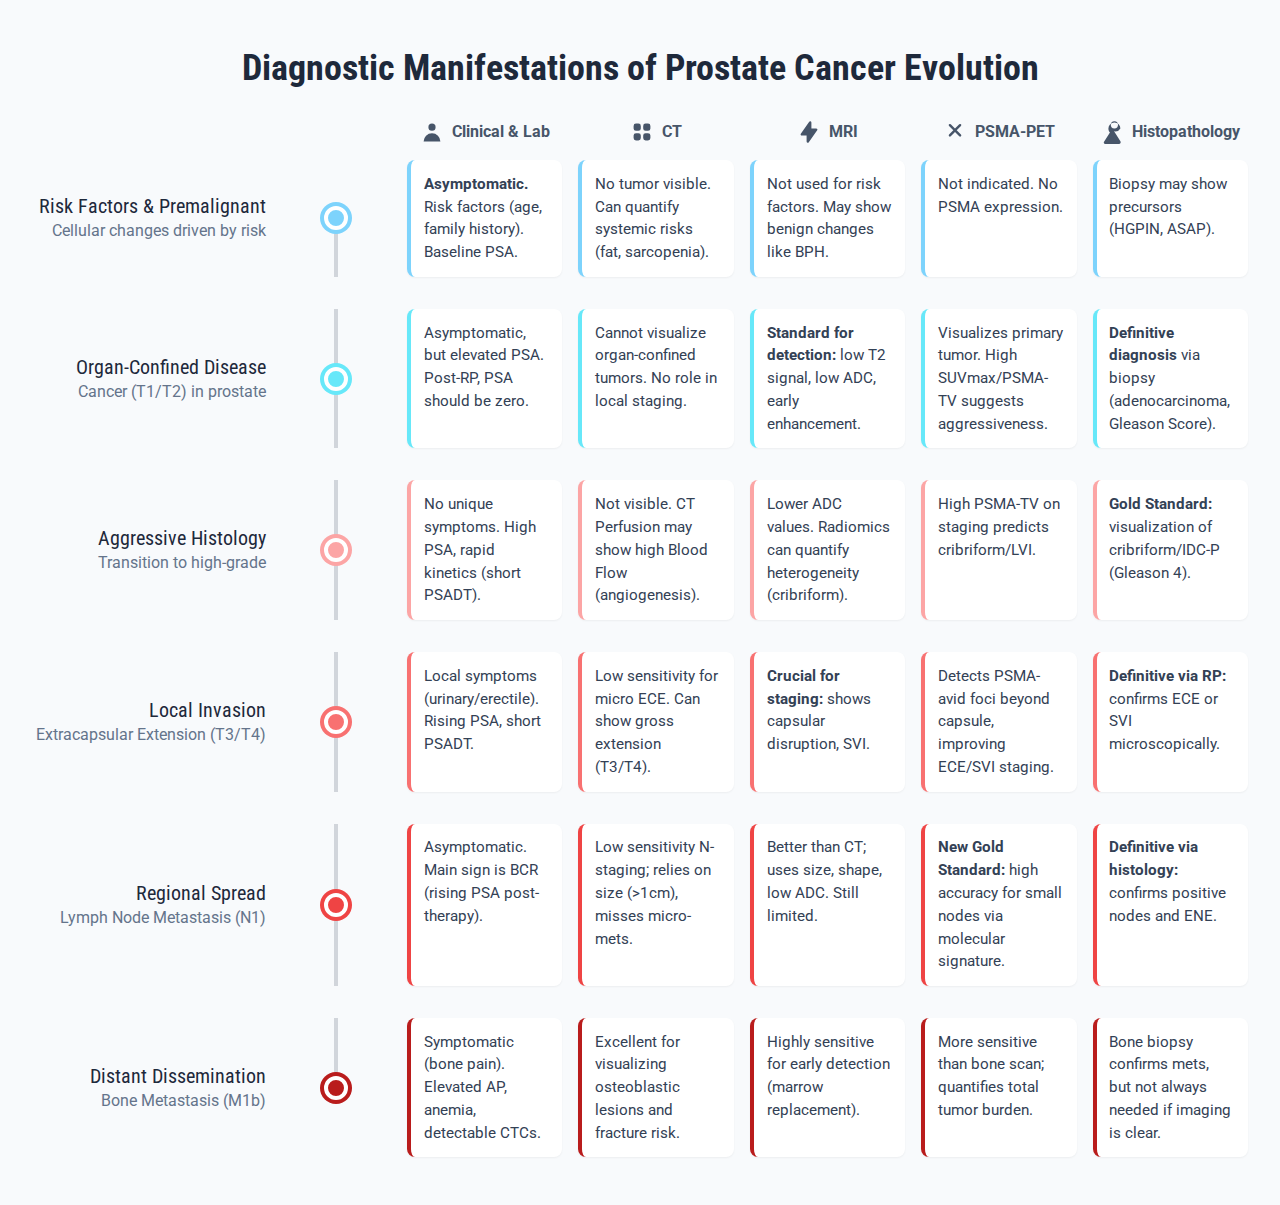
\includegraphics[width=\textwidth]{pe.png}
    \caption{The natural history of prostate cancer, illustrating the stages our model will learn.}
    \label{fig:prostate_evolution}
\end{figure}

\subsubsection{Stage 4: Translating Insight into Action: Generative Synthesis and Structured Reporting}
The final stage translates the model's learned representations into clinically actionable outputs. This includes generating high-fidelity images for any time point (past, present, or future) and for any counterfactual scenario, with a lightweight Diffusion Model used as a final post-processing step to add high-frequency detail and ensure clinical realism. Crucially, the model will generate structured radiological reports and tumor board recommendations using a \textbf{Transformer-based decoder}. This directly addresses the clinical need for clear, consistent, and efficient documentation, which is a major benefit of structured reporting that improves report quality, clarity, and standardization \cite{JorgHalfmann2023, SacoranskyKwan2024}. Our consortium's experience in creating LLM-based support apps and GUIs from structured reports ensures the successful implementation of this stage. The entire clinical workflow is depicted in Figure \ref{fig:workflow}.

\begin{figure}[H]
    \centering
    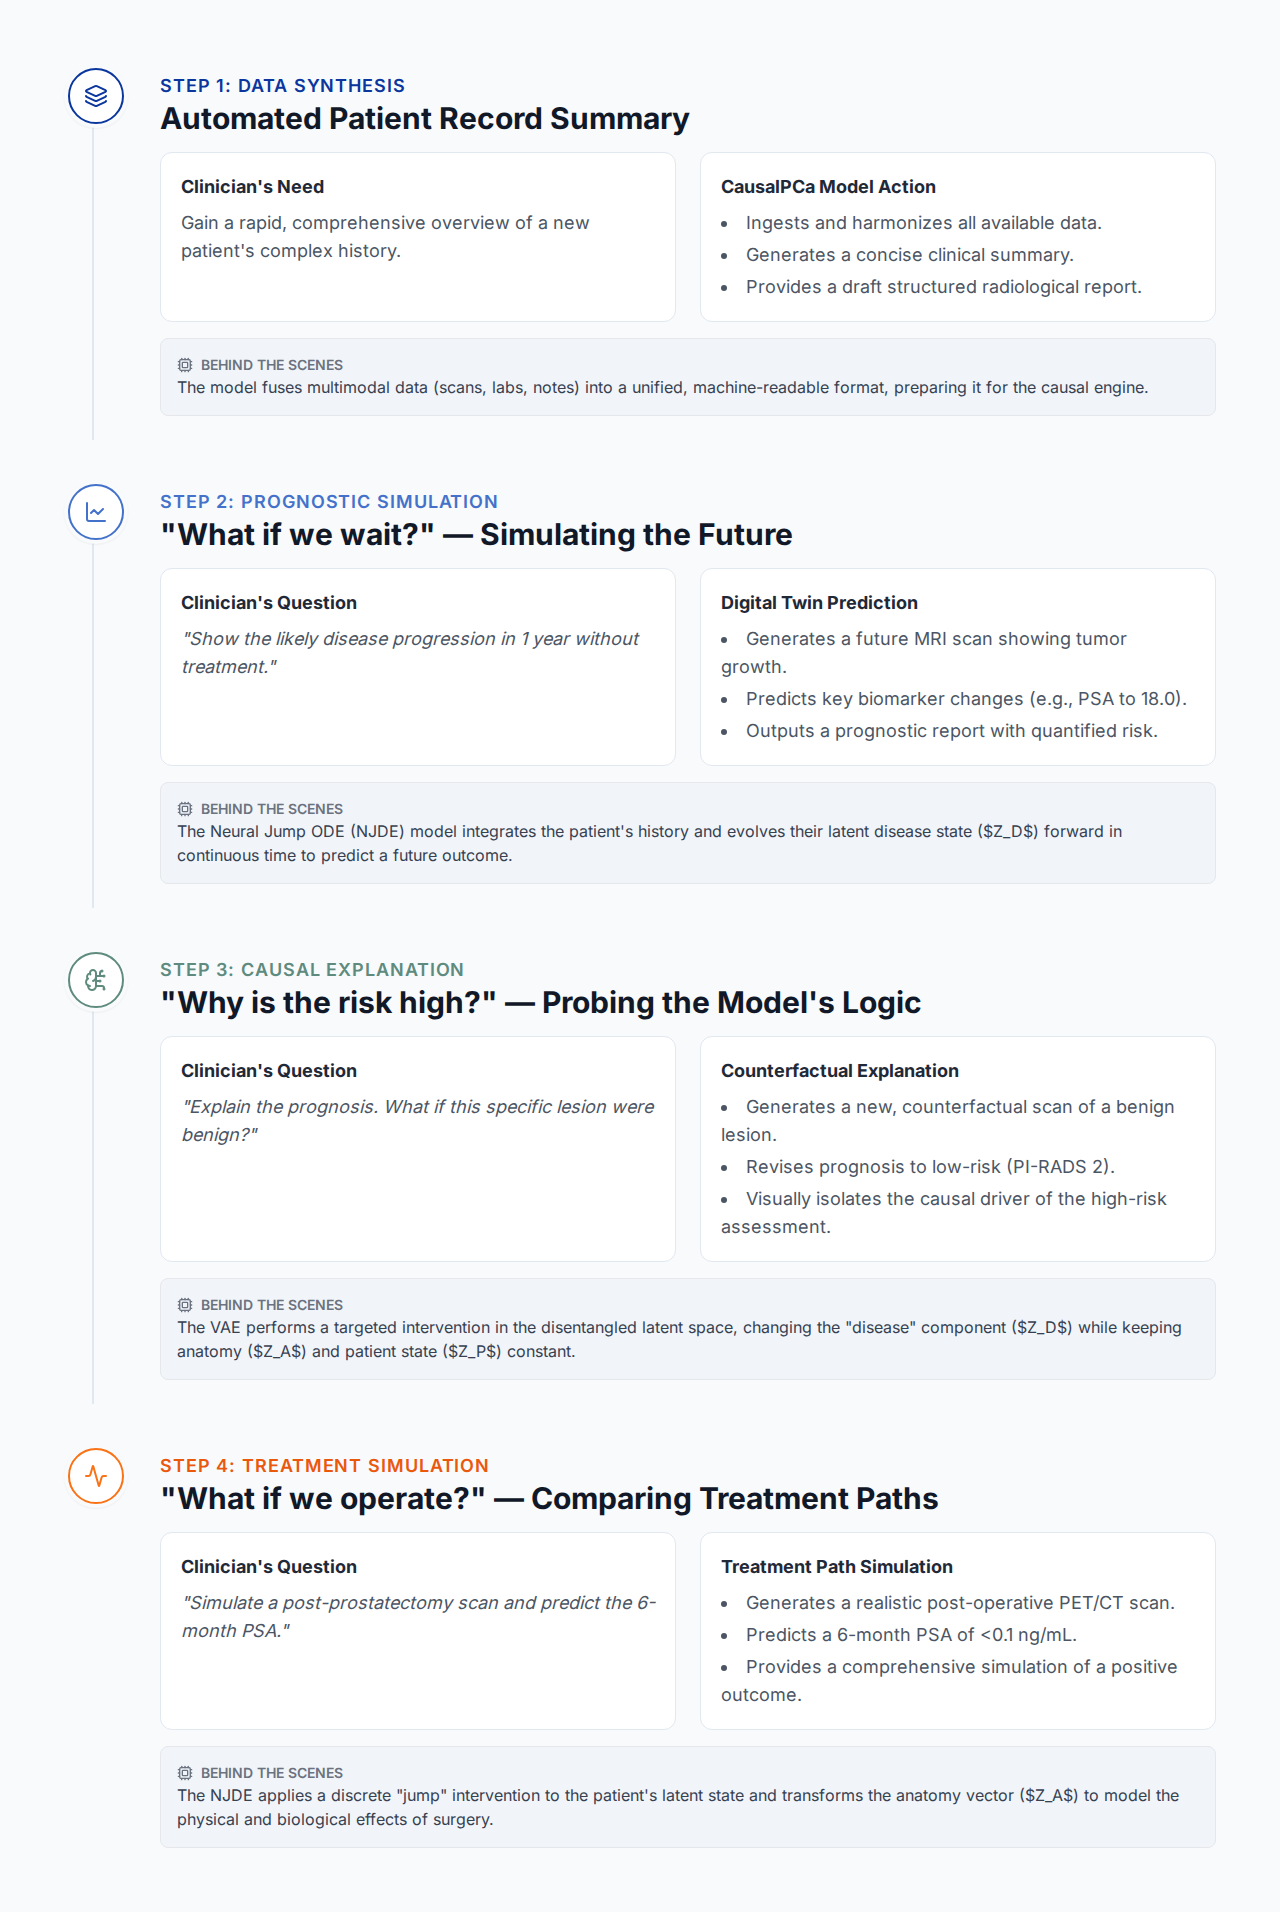
\includegraphics[width=\textwidth]{wf.png}
    \caption{The Multidisciplinary Workflow of Prostate Cancer Diagnosis: A complex, iterative process requiring multimodal data fusion and expert collaboration.}
    \label{fig:workflow}
\end{figure}

\subsection{Ambition}
The ambition of this project extends far beyond advancing the state-of-the-art in predictive modeling. We aim to establish a new paradigm for trustworthy AI in clinical medicine, shifting the focus from correlation to causation. By developing a model that can reason, simulate, and explain, we are creating a foundational technology with the potential for profound impact. This project will not only deliver a powerful tool for prostate cancer management but will also provide a blueprint for developing causal AI models in other complex disease areas. Our work will pioneer new methods for disentanglement, longitudinal modeling, and counterfactual reasoning that will be of immense value to the wider AI research community. The successful completion of this project will represent a significant step towards the realization of truly intelligent clinical decision support systems, paving the way for a future of more personalized, more effective, and more explainable medicine.

\subsection{Compliance with the EU Artificial Intelligence Act}
The proposed framework is designed from the ground up to align with the principles of trustworthy AI and to comply with the requirements for high-risk AI systems as laid down in the Regulation (EU) 2024/1689 (the "AI Act"). As a system intended for use in medical diagnosis and to guide treatment, it is classified as a \textbf{high-risk AI system} under Annex III of the Act. Our methodology directly addresses the core obligations for such systems:

\begin{itemize}
    \item \textbf{Risk Management System (Article 9):} Our project management (WP7) includes a continuous, iterative risk management process that will be maintained throughout the AI system's lifecycle. This involves identifying, analyzing, and mitigating known and reasonably foreseeable risks to health, safety, and fundamental rights, as mandated by Article 9.

    \item \textbf{Data and Data Governance (Article 10):} WP1 is entirely dedicated to establishing data governance practices that meet the quality criteria of Article 10. We will use relevant, representative, and error-free datasets. We will proactively implement measures to detect and mitigate potential biases through the disentanglement methods in Stage 2 and the confounder models in Stage 1. For the purpose of bias detection and correction, we will process special categories of personal data only where strictly necessary and with the appropriate safeguards as permitted under Article 10(5).

    \item \textbf{Technical Documentation and Record-Keeping (Articles 11 \& 12):} We commit to creating and maintaining comprehensive technical documentation as specified in Annex IV of the AI Act. Our system's design includes automatic logging capabilities to ensure traceability of operations, in compliance with the record-keeping requirements of Article 12.

    \item \textbf{Transparency and Provision of Information (Article 13):} A cornerstone of our project is to overcome the "black box" problem. The framework's ability to generate counterfactual explanations (Stage 4) is a direct implementation of the transparency requirements of Article 13. The system is designed so that its operations are sufficiently transparent to enable deployers to interpret its output and use it appropriately. We will provide detailed instructions for use that explain the system's capabilities, limitations, and the role of human oversight.

    \item \textbf{Human Oversight (Article 14):} The system is designed to augment, not replace, clinical experts. It functions as a decision support tool, ensuring that a natural person can oversee its functioning at all times. The design ensures that the user can understand the system's capabilities, monitor its operation, and decide to disregard, override, or reverse its output, fulfilling the requirements of Article 14.

    \item \textbf{Accuracy, Robustness, and Cybersecurity (Article 15):} WP5 is dedicated to rigorous validation of the model's accuracy and robustness. The system will be designed to be resilient against errors and inconsistencies through the disentanglement of confounders (Stage 2). We will implement robust cybersecurity measures to protect against vulnerabilities specific to AI, including data poisoning and adversarial attacks, as mandated by Article 15.
\end{itemize}

This principled approach ensures that our innovative framework is not only technologically advanced but also safe, trustworthy, and fully compliant with the Union's legal framework for artificial intelligence.


\subsection{State of the Art and the Need for a Causal Leap}
\subsubsection{The Clinical Frontier: Lutetium-177 PSMA Theranostics}
A key strength of this project is its foundation in a cutting-edge clinical environment defined by the use of Lutetium-177 PSMA (${}^{177}\text{Lu-PSMA-617}$) theranostics, a revolutionary and modern approach for managing metastatic castration-resistant prostate cancer (mCRPC). This paradigm combines therapy ("thera") and diagnostics ("nostics") by using a single molecular target—the Prostate-Specific Membrane Antigen (PSMA)—for both imaging and treatment, representing a new and very promising therapy \cite{HennrichEder2022}. PSMA is a protein that is highly overexpressed (up to 1,000-fold) on the surface of prostate cancer cells, making it an ideal target \cite{HennrichEder2022, LingBlois2022}.

The theranostic workflow is a form of personalized medicine. It begins with a diagnostic PET scan using a PSMA-targeting molecule labeled with a diagnostic radionuclide (e.g., Gallium-68). This scan precisely identifies PSMA-positive tumor locations, confirming that the patient is a suitable candidate for the therapy \cite{HennrichEder2022, KaewputVinjamuri2022}. If eligibility is confirmed, the patient is then treated with a nearly identical molecule, but this time labeled with a therapeutic radionuclide, Lutetium-177. The ${}^{177}\text{Lu}$ is a short-range beta-particle emitter that delivers highly targeted radiation directly to cancer cells, minimizing damage to surrounding healthy tissue \cite{HennrichEder2022, SadaghianiSheikhbahaei2022}.

This approach has proven to be a clinical breakthrough. The landmark Phase 3 VISION trial demonstrated that ${}^{177}\text{Lu-PSMA-617}$ significantly prolonged both overall survival (15.3 vs 11.3 months) and radiographic progression-free survival (8.7 vs 3.4 months) in patients with advanced mCRPC, leading to its FDA approval in 2022 \cite{TschanBorgna2022, ChandranFigg2022, RamnaraignSartor2023, JangKendi2023}. The therapy is not only effective but also has a favorable safety profile compared to traditional chemotherapy, with fewer grade 3 or 4 adverse events reported in the TheraP trial (33\% vs 53\%) \cite{HofmanEmmett2024, PatellKurian2023}.

Our project will leverage a unique dataset of paired diagnostic (PSMA PET/CT) and therapeutic (Lutetium-177 SPECT/CT) scans. This data provides an unparalleled opportunity to model the direct biological effects of a highly targeted and effective therapy, a critical component for building a robust causal model of disease progression and treatment response. Furthermore, because this therapy is administered at advanced stages, patients often have a rich, longitudinal history of prior treatments and imaging, providing the ideal data for our temporal models. The complexity of these cases also necessitates multidisciplinary tumor boards, giving us a unique opportunity to benchmark our model's recommendations against real-world expert consensus, making our consortium exceptionally well-suited for this project.

\subsubsection{The Unmet Need: Why Current AI Fails in the Clinical Workflow}
Despite the promise of AI, current models are fundamentally limited to pattern recognition and fail to understand the complex, dynamic, and causal nature of cancer. They cannot reason about the consequences of interventions, nor can they disentangle true disease progression from the myriad of confounders present in real-world data. This creates a critical gap between the technology's potential and its clinical utility. Clinicians need tools that can answer not just "what is the risk?" but "why is the risk high, and what can be done about it?". They need systems that can simulate and explain, not just predict. This project directly addresses this unmet need by developing a causal AI framework that can model the longitudinal trajectory of prostate cancer, providing a tool that is not only powerful but also trustworthy and aligned with the complex reasoning process of clinical experts.

\section{Impact}
The successful execution of this project will generate significant and lasting impact across multiple domains, from advancing the frontiers of science and technology to delivering tangible benefits for patients, clinicians, and the European innovation ecosystem. Our focus is not merely on creating a tool, but on establishing a new technological paradigm for clinical AI that is trustworthy, explainable, and directly aligned with the goals of the EU Cancer Mission and the strategic autonomy of the Union.

\subsection{Scientific and Technological Impact}
This project is poised to make fundamental contributions to the field of Artificial Intelligence and its application in medicine, directly addressing the EIC Pathfinder's goal to develop the scientific basis for breakthrough technologies.
\begin{itemize}
    \item \textbf{A New European Standard for Trustworthy Clinical AI:} We will pioneer a shift away from correlational "black-box" models towards truly causal and explainable AI. The development of a robust, generalizable framework for learning causal models from observational clinical data will represent a landmark achievement. This provides a blueprint for future research in a wide range of diseases and establishes a new European standard for the development and deployment of trustworthy AI systems in high-stakes environments, strengthening Europe's technological leadership.
    \item \textbf{Advancing the Frontier of Generative AI:} Our work on principled disentanglement, counterfactual generation, and longitudinal modeling with Neural Jump ODEs will push the boundaries of generative AI. By creating a model that can reason about cause and effect, we are developing a foundational technology with applications far beyond medicine, including in climate science, economics, and engineering. The novel techniques developed will be of immense value to the broader European AI community.
    \item \textbf{Fostering an Open and Sovereign European AI Ecosystem:} We are deeply committed to open science and Europe's digital sovereignty. We will make our code publicly available under a permissive open-source license. Crucially, we will contribute our curated, anonymized, and harmonized datasets to public repositories, with a specific focus on contributing to the \textbf{European Cancer Imaging (EUCAIM)} platform. This will not only foster further research and innovation across the EU but will also ensure that our work directly supports the development of a world-leading European data ecosystem for cancer research, reducing reliance on non-EU platforms.
\end{itemize}

\subsection{Societal and Clinical Impact}
The primary impact of this project will be the profound improvement in the management of prostate cancer, leading to better patient outcomes and more efficient, resilient healthcare systems across Europe.
\begin{itemize}
    \item \textbf{Enhanced Diagnostic Accuracy and Personalised Treatment:} By providing clinicians with a "digital twin" that can simulate disease trajectories and treatment responses, our framework will enable more accurate staging, better risk stratification, and truly personalized treatment planning. This will help to reduce both over- and under-treatment—a critical issue in prostate cancer—thereby minimizing treatment-related side effects and significantly improving patient quality of life.
    \item \textbf{Empowering Clinicians and Reducing Workload:} The model's ability to generate intuitive, counterfactual explanations ("what if this lesion were benign?") and automated structured reports will empower clinicians, augmenting their decision-making process and freeing up valuable time from tedious documentation. This will improve workflow efficiency, reduce burnout, and allow clinicians to focus on what matters most: patient care.
    \item \textbf{A Foundation for a New Era in European Oncology:} While focused on prostate cancer, the foundational technology developed in this project is modality-agnostic and disease-agnostic. It has the potential to be adapted to other cancers (e.g., breast, lung) and complex chronic diseases, paving the way for a new era of data-driven, causal medicine that is more personalized, more effective, and more explainable, with Europe at the forefront.
\end{itemize}

\subsection{Dissemination, Communication, and Exploitation}
We are committed to maximizing the impact of this project through a comprehensive dissemination, communication, and exploitation strategy designed to engage stakeholders at all levels and create new market opportunities.
\begin{itemize}
    \item \textbf{High-Impact Scientific Publications:} We will publish our methodological advancements and clinical validation results in leading peer-reviewed journals (e.g., Nature Machine Intelligence, The Lancet Digital Health, Medical Image Analysis) and present at premier international conferences (e.g., MICCAI, NeurIPS, RSNA).
    \item \textbf{Open Source and Open Data:} As stated, all code will be open-sourced via European platforms. Our curated, anonymized datasets will be contributed to public repositories, including a dedicated contribution to the \textbf{European Cancer Imaging (EUCAIM)} platform, to ensure our data legacy strengthens the European research community.
    \item \textbf{Engagement with the Clinical and Patient Community:} We will actively engage with European clinical societies (e.g., EAU, ESMO) and patient advocacy groups (e.g., Europa Uomo) through workshops, webinars, and presentations. This ensures our work is aligned with real-world clinical needs and facilitates its translation into clinical practice across the EU.
    \item \textbf{Commercial Exploitation and Standardization:} We will explore pathways for commercial exploitation through partnerships with European medical imaging companies and health-tech startups, creating new market opportunities within the Union. Furthermore, we will actively participate in standardization bodies to promote the adoption of our structured reporting and causal AI frameworks as a new European standard for trustworthy clinical AI.
\end{itemize}

\section{Implementation}

\subsection{Work Plan and Consortium}
The project will be executed over 36 months, organized into seven interconnected Work Packages (WPs). The detailed timeline, deliverables (D), and milestones (M) are visualized in the Gantt chart (Figure \ref{fig:gantt}).

\begin{figure}[H]
    \centering
    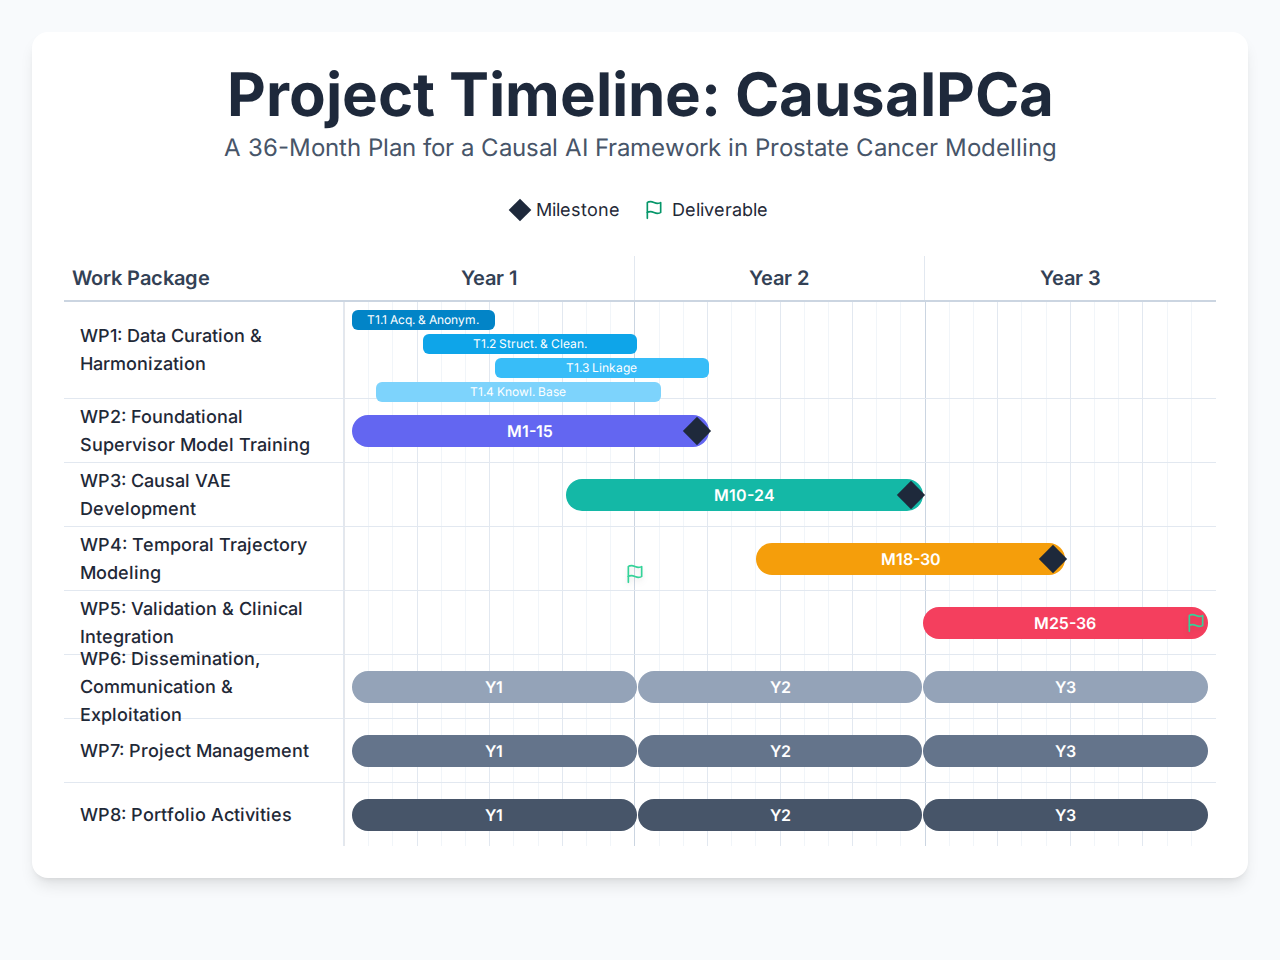
\includegraphics[width=\textwidth]{gantt.png}
    \caption{Project Gantt Chart illustrating the timeline, work packages, milestones, and deliverables.}
    \label{fig:gantt}
\end{figure}

\begin{itemize}
    \item \textbf{WP1: Data Curation and Harmonization (Months 1-9).} Led by Universitätsklinik für Radiologie und Nuklearmedizin. This WP involves aggregating the proprietary multi-center cohort, integrating public datasets (TCGA-PRAD, ProstateNET), and performing rigorous data harmonization, including DICOM to NIFTI conversion, pseudonymization, and image normalization. \textit{(D1.1: Curated, harmonized dataset)}.
    \item \textbf{WP2: Foundational Supervisor Model Training (Months 4-15).} This WP will focus on developing and validating the suite of expert supervisor models (ordinal classifiers, survival regressor, confounder models) that will provide the strong inductive biases for the main generative framework.
    \item \textbf{WP3: Causal VAE Development (Months 10-24).} The core of this WP is the training of the disentangled Variational Autoencoder, leveraging the supervisors from WP2 to enforce causal separation of anatomy, disease, and confounder latent spaces.
    \item \textbf{WP4: Temporal Trajectory Modeling (Months 18-30).} This WP will implement and train the Neural Jump ODE on the disentangled disease vectors from WP3 to model longitudinal patient trajectories, including the impact of interventions.
    \item \textbf{WP5: Validation and Clinical Integration (Months 25-36).} This WP will conduct the comprehensive evaluation of the final model, including quantitative metrics, uncertainty quantification, and the clinician-in-the-loop study to assess real-world utility and impact on workflow.
    \item \textbf{WP6: Dissemination, Communication, and Exploitation (Months 1-36).} This continuous WP covers all project outreach, including publications, conference presentations, open-source code releases, and engagement with clinical and patient communities.
    \item \textbf{WP7: Project Management (Months 1-36).} This WP ensures the smooth execution of the project, managing timelines, resources, and reporting. The project will be led by a principal investigator with dual expertise in clinical radiology and artificial intelligence, ensuring a seamless bridge between the technical and clinical aspects of the project.
\end{itemize}

\subsection{Data Sources and Cohort}
A key strength of this proposal is the direct access to already preprocessed, rich, longitudinal, and multimodal data from the applicants’ own clinical institutions and established collaborators. This will form the core training dataset, which can be expanded with new cases during the project from our own or collaborating institutions. An ethical approval for using the preprocessed data for scientific purposes has already been obtained.

\subsubsection{Proprietary Multi-Center Clinical Cohort}
\begin{itemize}
    \item \textbf{Universitätsklinik für Radiologie und Nuklearmedizin (Magdeburg):} As the lead applicant institution, the clinic will provide a rich dataset from its patient care archives. This includes:
    \begin{itemize}
        \item Approximately 150-200 longitudinal studies of patients with paired baseline PSMA-PET/CT and mpMRI scans for primary staging and follow-up.
        \item A unique cohort of approximately 150 patients with advanced disease who have undergone Lutetium-177 PSMA radioligand therapy (RLT). For these patients, we have paired pre-therapy PSMA-PET/CT scans and post-therapy Lutetium SPECT/CT scans, which are essential for modeling treatment response.
        \item A very unique cohort of interim therapy controls based on PSMA-PET/CT and CT –pairs from 40 patients.
    \end{itemize}
    \item \textbf{Abteilung für Nuklearmedizin | Universitätsmedizin Halle:} This collaborating institution cans provide a comparable dataset, enriching the cohort’s geographical and technical diversity. It is expected to contribute:
    \begin{itemize}
        \item Approximately 100 additional paired PSMA-PET/CT and mpMRI studies.
        \item Approximately 100 additional paired pre-therapy PSMA-PET/CT and post-therapy Lutetium SPECT/CT studies.
    \end{itemize}
    \item \textbf{Klinik für Nuklearmedizin | Universitätsmedizin Charite:} This collaborating institution cans provide a comparable dataset, enriching the cohort’s geographical and technical diversity. It is expected to contribute:
    \begin{itemize}
        \item Approximately 100 additional paired PSMA-PET/CT and mpMRI studies.
        \item Approximately 300 additional paired pre-therapy PSMA-PET/CT and post-therapy Lutetium SPECT/CT studies.
    \end{itemize}
    \item \textbf{Radiological Practice Rad. Sudenburg – ambulatory care (Magdeburg):} This collaboration provides access to a significant number of high-quality diagnostic scans from a external practice setting, further enhancing the dataset’s diversity.
    \begin{itemize}
        \item Approximately 200 CT and mpMRI studies for diagnosis and active surveillance.
    \end{itemize}
\end{itemize}
This combined proprietary cohort of over 1000 patients, with its unique inclusion of post-RLT SPECT/CT data, provides an unparalleled resource for training a model capable of understanding the entire spectrum of prostate cancer progression and treatment.

\subsubsection{Integration with Public Datasets}
To augment our proprietary data, enhance statistical power, and rigorously test the generalizability of our models, we will integrate several large, well-curated public datasets. These have been chosen to cover a wide range of clinical scenarios, imaging modalities, and patient populations.
\begin{itemize}
    \item \textbf{The Cancer Genome Atlas Prostate Adenocarcinoma (TCGA-PRAD):} This will serve as a primary resource for linking our imaging-based models to underlying genomic data. Its rich, multi-modal imaging (MRI, CT, PET) and detailed clinical and genomic information are ideal for validating our model’s biological grounding.
    \item \textbf{ProstateNET (EUCAIM):} Specifically, we will leverage the UC8 dataset for active surveillance, which contains longitudinal MRI and PSA data. This aligns with the European Union’s goal of fostering a shared cancer imaging infrastructure.
    \item \textbf{NAF-PROSTATE:} This dataset provides systematic longitudinal PET/CT data for patients with bone metastases, which will be invaluable for validating the temporal modeling of our framework (WP4) in an advanced disease setting.
\end{itemize}
This combined data strategy provides an unparalleled foundation for this high-risk, high-gain project, mitigating the risk of data scarcity and ensuring the developed technology is robust, validated, and ready for broader clinical application.

\textbf{Data Governance and AI Act Compliance (Article 10):} All data will be managed within a secure, federated learning-ready environment based on the XNAT platform, ensuring robust data hosting and management. Our data governance framework is designed to meet the stringent quality criteria of Article 10 of the EU AI Act. The data collection is overseen by our clinical partners, and all data undergoes a rigorous curation and verification process by trained clinicians to ensure it is relevant, representative, and as free of errors as possible. To address potential biases, our disentanglement methods (Stage 2) and confounder models (Stage 1) are designed to detect and mitigate biases related to demographics and acquisition hardware. For the purpose of bias detection and correction, we will process special categories of personal data only where strictly necessary and with the appropriate safeguards as permitted under Article 10(5), ensuring our dataset is suitable for training a high-risk AI system. All data will be handled in strict compliance with GDPR and ethical guidelines.

\subsection{Illustrative Clinical Workflow}
To make the vision concrete, consider the following illustrative workflow of a clinician using the fully trained CausalPCa tool for a new patient:
\begin{enumerate}
    \item \textbf{Automated Patient Summary:} The model ingests the patient's entire record—including scans, lab results, and notes—and generates a concise summary, including a draft structured report for the latest scan. This saves the clinician significant pre-reading time.
    \item \textbf{Prognostic Inquiry:} The clinician, concerned about a suspicious lesion, asks the system via a simple interface, \textit{"Show prognosis in 1 year without treatment."}
    \begin{itemize}
        \item \textbf{Model Action:} The NJDE integrates the patient's history and solves its learned continuous differential equation forward in time to predict the disease state ($Z_D$) at $t+1$ year.
        \item \textbf{Model Output:} The tool generates a future MRI showing likely tumor progression, a predicted PSA of 18.0 ng/mL, and an accompanying prognostic report highlighting the increased risk.
    \end{itemize}
    \item \textbf{Explainable Reasoning Inquiry:} To understand the basis for the high-risk prediction, the clinician probes the model's reasoning by asking, \textit{"What if the primary lesion were benign?"}
    \begin{itemize}
        \item \textbf{Model Action:} The model performs a targeted intervention on the latent space, setting the disease component corresponding to the lesion to a "healthy" state while keeping all other patient factors constant.
        \item \textbf{Model Output:} It generates a new, counterfactual image where the lesion appears benign, along with a revised, low-risk prognostic report and a PI-RADS 2 classification. This visual and textual explanation gives the clinician confidence in the model's assessment.
    \end{itemize}
    \item \textbf{Treatment Planning Inquiry:} The clinician now considers surgery and asks, \textit{"Simulate a post-prostatectomy PET scan and predict the 6-month PSA."}
    \begin{itemize}
        \item \textbf{Model Action:} The model applies a "prostatectomy" intervention. This triggers a learned discrete \textbf{jump} in the NJDE to an immediate post-operative disease state. Simultaneously, a transformation is applied to the anatomy vector $Z_A$ to model the physical removal of the prostate. The NJDE then evolves this new state forward for 6 months.
        \item \textbf{Model Output:} It generates a realistic post-operative PET/CT scan and provides a predicted 6-month PSA value of <0.1 ng/mL, offering a comprehensive simulation of a positive treatment outcome.
    \end{itemize}
\end{enumerate}

\subsection{Evaluation and Validation}
The project's success will be measured through a rigorous, multi-faceted evaluation plan that combines quantitative metrics with qualitative, clinician-in-the-loop studies to assess real-world utility and trustworthiness.

\subsubsection{Quantitative Metrics}
Model performance will be assessed using a comprehensive suite of metrics tailored to each sub-task:
\begin{itemize}
    \item \textbf{Supervisor Model Performance:}
        \begin{itemize}
            \item \textbf{Classification:} Accuracy, Area Under the Curve (AUC), F1-Score, and Quadratic Weighted Kappa for ordinal tasks.
            \item \textbf{Survival Regression:} Concordance Index (C-index) and Mean Absolute Error on censored data.
        \end{itemize}
    \item \textbf{Generative Model Performance:}
        \begin{itemize}
            \item \textbf{Image Generation Quality:} Fréchet Inception Distance (FID), Structural Similarity Index (SSIM), and Learned Perceptual Image Patch Similarity (LPIPS) to measure realism and fidelity \cite{VigneshwaranOhara2024, Singla2022}.
            \item \textbf{Counterfactual Quality:} We will use a comprehensive suite of metrics to assess axiomatic soundness (effectiveness, composition, reversibility) \cite{KomanduriWu2023, MonteiroRibeiro2023}, validity (success rate of flipping a classifier’s decision) \cite{SinglaEslami2021, Singla2022}, proximity (distance to the original), and realism (FID) \cite{GuoDeng2024}.
        \end{itemize}
\end{itemize}

\subsubsection{Uncertainty Quantification}
A key feature for clinical trust is the model's ability to quantify its own uncertainty. Our VAE-based architecture is intrinsically probabilistic and allows for robust uncertainty quantification. We will employ two complementary methods:
\begin{itemize}
    \item \textbf{Latent Space Sampling:} For a given input, we will draw multiple samples from its learned latent distribution. The variance in the resulting predictions will serve as a robust measure of the model's epistemic uncertainty \cite{BustinMeyer2025}.
    \item \textbf{Direct Variance Utilisation:} The variance vector $\sigma^2$ produced by the VAE encoder is a direct indicator of feature-level uncertainty. We will concatenate this variance vector to the mean vector as a direct input to downstream models, allowing them to learn to depend more on high-confidence features \cite{FriedrichFrisch2024}.
\end{itemize}

\subsubsection{Clinical Plausibility and Workflow Integration Study}
Beyond quantitative metrics, a practical, clinician-in-the-loop study is essential to assess the model's real-world utility and trustworthiness.
\begin{itemize}
    \item \textbf{Assessing Counterfactual Plausibility and Usefulness:} To evaluate the quality of our generated explanations, we will conduct a human-grounded study with radiologists and oncologists. Clinicians will be presented with a series of cases, each including an original image and its corresponding model-generated counterfactual (e.g., an image of a tumorous prostate and its benign-looking counterfactual). They will score the counterfactuals on a Likert scale for:
    \begin{itemize}
        \item \textbf{Clinical Plausibility:} Does the generated image appear realistic and anatomically sound?
        \item \textbf{Usefulness for Explanation:} Does the visual difference between the original and counterfactual image provide a clear and understandable reason for the model's prediction?
    \end{itemize}
    \item \textbf{Measuring Workflow Improvement with Structured Reports:} To assess the impact of the automated reports, we will perform a comparative workflow study. A control group of clinicians will review patient cases using traditional free-text reports and standard image viewers. An experimental group will review the same cases using our system's auto-generated structured reports and prognostic visualizations. We will measure:
    \begin{itemize}
        \item \textbf{Efficiency:} Time taken to extract key information (e.g., TNM stage, PI-RADS score, presence of key findings) required for treatment planning.
        \item \textbf{Accuracy and Concordance:} Inter-rater agreement and accuracy of the extracted information compared to an expert-defined ground truth.
        \item \textbf{User Satisfaction:} Clinicians' perceived efficiency, clarity, and confidence in their decisions will be assessed using a standardized questionnaire (e.g., the System Usability Scale).
    \end{itemize}
\end{itemize}

\subsection{Risk Analysis, Mitigation, and AI Act Compliance}
This is an ambitious, high-risk project at the frontier of AI research. We have identified the primary risks and have developed clear mitigation strategies that are intrinsically linked to our compliance with the EU AI Act. Our risk management process, as detailed in WP7, is continuous and iterative, designed to address risks to health, safety, and fundamental rights throughout the AI system's lifecycle, in direct alignment with \textbf{Article 9} of the Act. Furthermore, our methodology is designed to comply with the ‘do no significant harm’ principle as per Article 17 of the EU Taxonomy Regulation, ensuring our research does not negatively impact environmental objectives.

\begin{itemize}
    \item \textbf{Risk 1: Training Instability and Data Scalability.} The complexity of the proposed model presents a risk of training instability, especially given the multi-modal, multi-stage nature of the framework.
    \item \textbf{Mitigation:} Our primary mitigation is the \textbf{sequential, multi-stage training framework}. By decomposing a single, intractable optimization problem into a series of manageable sub-problems, we enhance stability and improve data efficiency. This modularity, a cornerstone of our design, allows us to isolate and troubleshoot issues at specific stages, a process our team has successfully employed in past projects involving synthetic image generation and predictive modeling.

    \item \textbf{Risk 2: Generalizability and Overfitting to Spurious Correlations.} AI models are prone to learning shortcuts from site-specific or technical artifacts in the data, limiting their real-world performance and clinical trustworthiness.
    \item \textbf{Mitigation (AI Act Articles 10 \& 15):} Our framework is built on \textbf{principled disentanglement}. By explicitly separating style and confounder variables ($Z_S$) from disease variables ($Z_D$) and embedding strong domain knowledge as inductive biases (e.g., ordinal losses), we guide the model to learn the true causal factors of the disease. This directly addresses the need for robustness and accuracy under Article 15. The multi-center nature of our dataset, combined with our data governance practices (see Data Sources and Cohort section), ensures we meet the data quality requirements of Article 10.

    \item \textbf{Risk 3: Performance with Incomplete and Heterogeneous Data.} Real-world clinical data is inherently "messy," with missing modalities and irregular time points, which can severely hamper model performance.
    \item \textbf{Mitigation:} Our framework directly confronts this through its \textbf{Neural Jump ODE architecture}, which is inherently designed to handle sparse, irregularly sampled data. The use of a \textbf{masked loss function} during NJDE training is a key technique that allows the model to learn from all available data without being penalized for missingness, thereby turning the heterogeneity of the data from a weakness into a strength.

    \item \textbf{Risk 4: Clinical Trustworthiness and the "Black Box" Problem.} For any AI tool to be adopted, clinicians must trust its outputs and understand its reasoning.
    \item \textbf{Mitigation (AI Act Articles 13 \& 14):} Our primary strategy for building trust is \textbf{explainability through counterfactuals}. This mechanism allows clinicians to probe the model's reasoning by asking "what-if" questions, transforming it from an opaque oracle into an interactive and verifiable partner. This directly implements the transparency requirements of Article 13. The system is designed as a decision support tool, ensuring a clinician is always in control (\textbf{human oversight}, Article 14). The design, as shown in the "Illustrative Clinical Workflow," ensures the user can understand, override, and reverse the system's outputs.
\end{itemize}
Furthermore, comprehensive \textbf{technical documentation} will be maintained throughout the project as specified in Annex IV of the AI Act, and our system's design includes automatic logging capabilities to ensure traceability of operations, in compliance with the record-keeping requirements of \textbf{Articles 11 and 12}.

\subsubsection{Cybersecurity and Model Integrity}
Securing a multimodal health AI application requires a multi-layered, comprehensive security strategy that addresses AI-specific threats, ensures patient data privacy, and enforces strict regulatory compliance. The integration of image diagnostics and clinical text analytics in AI models introduces complex vulnerabilities, as Convolutional Neural Networks (CNNs) are susceptible to image-based adversarial attacks, while models processing textual EHR data can also be manipulated. Here are the critical strategies for securing such a multimodal AI application:

\paragraph{1. Enhancing AI Model Robustness and Integrity}
To defend the integrity and reliability of the machine learning models against malicious inputs and training manipulations:
\begin{itemize}
    \item \textbf{Implement Adversarial Defense Mechanisms:} Adopting defensive strategies significantly increases model resilience. This includes methods like adversarial training, defensive distillation, and hybrid defenses.
    \item \textbf{Mitigate Data Poisoning:} Proactive scans will be implemented to identify corrupted data and protect training pipelines from data poisoning attacks.
    \item \textbf{Stress Testing and OOD Detection:} We will conduct rigorous stress tests to validate the model's robustness under adversarial inputs and implement Out-of-Distribution (OOD) detection to flag inputs that fall outside the model's expected data range.
    \item \textbf{Data Quality Assessment:} We will perform thorough checks on training datasets for completeness, consistency, and correctness to avoid low performance.
\end{itemize}

\paragraph{2. Ensuring Data Confidentiality and Privacy}
Given that the application handles sensitive patient data, robust measures must be in place to prevent privacy violations:
\begin{itemize}
    \item \textbf{Federated Learning (FL):} We will utilize FL frameworks to allow collaborative training of AI models across distributed healthcare nodes without transferring raw patient data.
    \item \textbf{Differential Privacy (DP):} We will integrate DP mechanisms to introduce calculated noise into computations, providing a guaranteed maximum privacy loss.
    \item \textbf{Encryption and Secure Protocols:} We will employ end-to-end encryption and use secure cloud storage solutions that adhere to standards like HIPAA and GDPR.
    \item \textbf{Minimize Data Leakage:} We will address the vulnerability of deep learning models to inadvertently expose sensitive training data, using techniques like disentangled representations.
\end{itemize}

\paragraph{3. Operational, Transparency, and Regulatory Frameworks}
Securing the application also requires comprehensive governance:
\begin{itemize}
    \item \textbf{Multi-layered Security Architecture:} We will adopt a holistic strategy across the system architecture, integrating security at the edge, fog, and cloud layers.
    \item \textbf{Continuous Monitoring and Anomaly Detection:} We will implement continuous model monitoring to identify anomalous model behaviours in real-time.
    \item \textbf{eXplainable Artificial Intelligence (XAI):} Mechanisms such as SHAP or LIME will be integrated to explain how the AI model generates its output.
    \item \textbf{Audit Trail:} We will maintain a complete audit trail that logs every user action, system access, and prediction.
    \item \textbf{Human Oversight (Clinicians Double-Check):} We will implement mechanisms that require confirmation by the healthcare professional before sending a clinical case to the AI system.
    \item \textbf{Bias Check and Fairness:} We will explicitly check for and mitigate algorithmic bias inherited from training datasets.
    \item \textbf{Regulatory Compliance and AI Passport:} We will ensure the application adheres strictly to standards like the NIST Cybersecurity Framework, HIPAA, and GDPR, and maintain an AI Passport documenting the system's purpose, training, and potential biases.
\end{itemize}


\bibliographystyle{unsrt}
\bibliography{bibl}

\end{document}